\section{Results and Discussion}

\begin{figure}[h]
\centering
\begin{tabular}{cc}
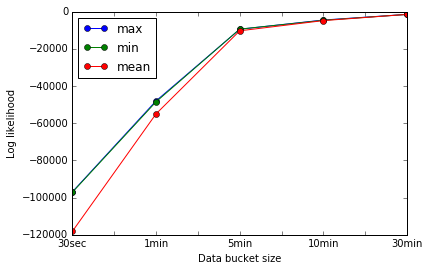
\includegraphics[width=.4\linewidth]{figs/physical_loglikelihood} & 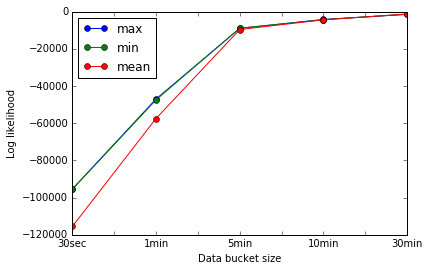
\includegraphics[width=.4\linewidth]{figs/full_loglikelihood} \\
(a) Physical Graph IPF Log Likelihoods & (b) Fully-connected Graph IPF Log Likelihoods \\[6pt]
\end{tabular}
\caption{Plots of the log-likelihood of the IPF runs on the physical and fully-connected graph across different bucket sizes and bucket aggregation functions. We can see that at as the amount of aggregation increases, the log-likelihood increases, and the choice of aggregation function matters less. This is in line with what we would expect, but the converged parameters in the coarser cases may lose some of the subtle interactions between microzones.
It is also interesting to note that the log-likelihoods of the physical and fully-connected graphs are very similar.}
\label{fig:loglikelihood}
\end{figure}

In this section, we discuss the results from running IPF over the two MRF graphical structures representing the microzones in the south-west corner of Soda Hall's AMPlab.

\subsection{Data Aggregation and Log-Likelihood}

Because we were not sure what method and degree of aggregation would perform best for our task, we explored various degrees and types of aggregation.
The resulting log-likelihoods from converged IPF runs over the two graphs are illustrated in Figure~\ref{fig:loglikelihood}.
While the \texttt{mean} aggregation function consistently results in lower log-likelihoods for all window sizes in both graphs, the log-likelihoods to converge to very similar values (-1494, -1504, -1488 for \texttt{mean}, \texttt{min} and \texttt{max} for 30-minute window aggregation on the physical graph, for example) with higher degrees of aggregation, regardless of the choice of function.
Also interesting is the fact that both the fully-connected and physical graphs have similar log-likelihoods.
At the 30-minute aggregation level, the fully-connected graph has a log-likelihood about 100 higher than that of the physical graph, but as we will discuss below, this higher log-likelihood does not actually correlate with a more useful set of parameters.

\subsection{Edge Parameters}

\begin{figure}[ht]
\centering
\begin{tabular}{cccc}
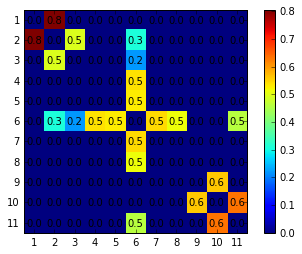
\includegraphics[width=1.3in]{figs/30minmin00conf} & 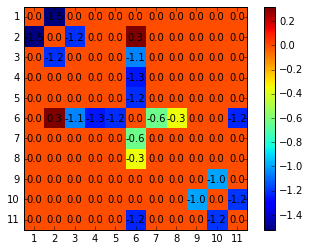
\includegraphics[width=1.3in]{figs/30minmin01conf} & 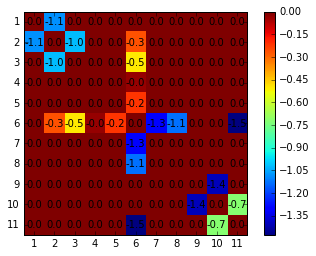
\includegraphics[width=1.3in]{figs/30minmin10conf} & 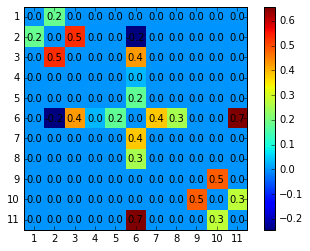
\includegraphics[width=1.3in]{figs/30minmin11conf} \\
(a) (0,0) & (b) (0,1) & (c) (1,0) & (d) (1,1) \\[6pt]
\end{tabular}
\caption{Edge potentials for the IPF run using 30 minute buckets (aggregated using \texttt{min}) in the physically connected Soda AMPlab graph (Figure~\ref{fig:soda_edges}(a)). This model had the \emph{highest} log-likelihood of the IPF run on the physical graph.}
\label{fig:30minminphysical}
\end{figure}

\begin{figure}[ht]
\centering
\begin{tabular}{cccc}
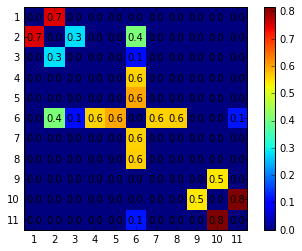
\includegraphics[width=1.3in]{figs/30secmin00conf} & 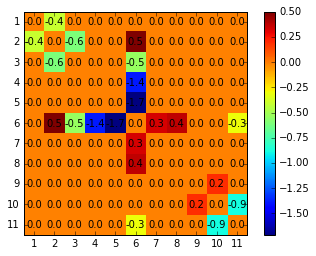
\includegraphics[width=1.3in]{figs/30secmin01conf} & 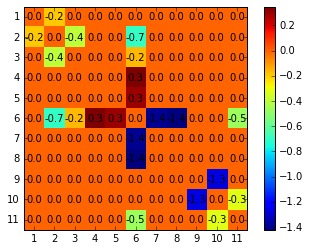
\includegraphics[width=1.3in]{figs/30secmin10conf} & 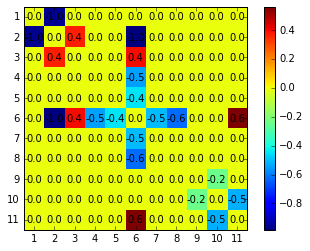
\includegraphics[width=1.3in]{figs/30secmin11conf} \\
(a) (0,0) & (b) (0,1) & (c) (1,0) & (d) (1,1) \\[6pt]
\end{tabular}
\caption{Edge potentials for the IPF run using 30 second buckets (aggregated using \texttt{min}) in the physically connected Soda AMPlab graph (Figure~\ref{fig:soda_edges}(a)). This model had the \emph{lowest} log-likelihood of the IPF run on the physical graph.}
\label{fig:30secminphysical}
\end{figure}

\begin{figure}[ht]
\centering
\begin{tabular}{cccc}
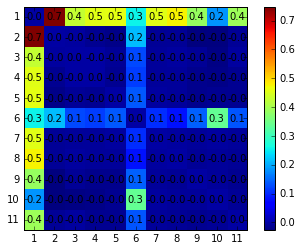
\includegraphics[width=1.3in]{figs/30secmin00fullconf} & 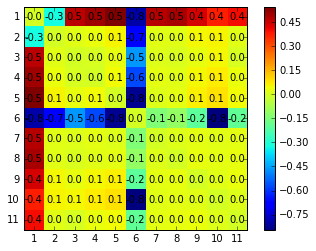
\includegraphics[width=1.3in]{figs/30secmin01fullconf} & 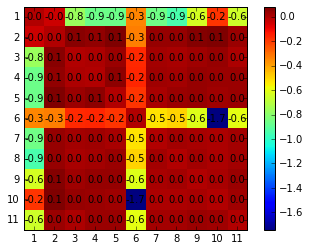
\includegraphics[width=1.3in]{figs/30secmin10fullconf} & 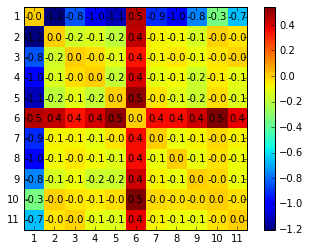
\includegraphics[width=1.3in]{figs/30secmin11fullconf} \\
(a) (0,0) & (b) (0,1) & (c) (1,0) & (d) (1,1) \\[6pt]
\end{tabular}
\caption{Edge potentials for the IPF run using 30 second buckets (aggregated using \texttt{min}) in the fully-connected Soda AMPlab graph (Figure~\ref{fig:soda_edges}(b)). This model had the \emph{lowest} log-likelihood of the IPF run on the fully-connected graph.}
\label{fig:30secminfull}
\end{figure}

\begin{figure}[ht]
\centering
\begin{tabular}{cccc}
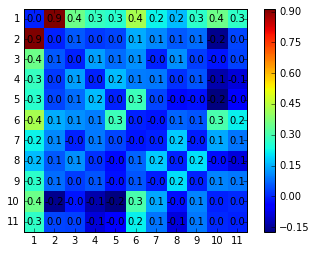
\includegraphics[width=1.3in]{figs/30minmin00fullconf} & 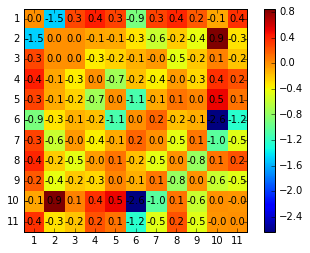
\includegraphics[width=1.3in]{figs/30minmin01fullconf} & 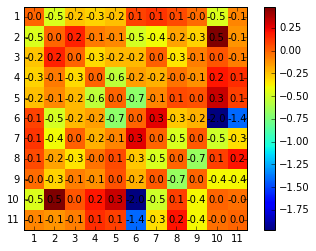
\includegraphics[width=1.3in]{figs/30minmin10fullconf} & 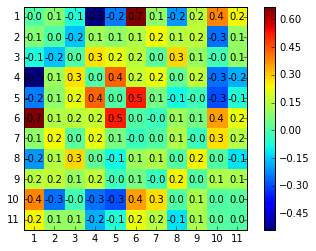
\includegraphics[width=1.3in]{figs/30minmin11fullconf} \\
(a) (0,0) & (b) (0,1) & (c) (1,0) & (d) (1,1) \\[6pt]
\end{tabular}
\caption{Edge potentials for the IPF run using 30 minute buckets (aggregated using \texttt{min}) in the fully-connected Soda AMPlab graph (Figure~\ref{fig:soda_edges}(b)). This model had the \emph{highest} log-likelihood of the IPF run on the fully-connected graph.}
\label{fig:30minminfull}
\end{figure}


After running IPF, we get back an array of $2\times 2$ matrices, each representing an edge parameter from the graphical structure.
For each element in the pairwise edge parameter matrix --- (0,0), (0,1), (1,0) and (1,1) --- we plot the confusion matrix for all edges in the graph (Figures ~\ref{fig:30secminphysical}\ref{fig:30secminfull}\ref{fig:30minminphysical}\ref{fig:30minminfull}).
We now give a brief overview of what we expect to find in each of these matrices:

\begin{itemize}[noitemsep,nolistsep]
\item (0,0): The more positive an entry in this matrix is, the stronger the thermal \emph{cooling} coupling between the two microzones. 
If an entry is low (or negative), then this likely means that one of the zones tends to retain heat rather than dissipate it (which may be due to the HVAC system).
\item (0,1) and (1,0): These two matrices represent the strength of the negative coupling between two microzones, that is, how likely is it that one will heat and one will cool in the same time window.
We expect to see mainly negative values here; there are no strong physical mechanisms that would cause a strong inverse thermal connection between two microzones.
Small values (either positive or negative) suggest that the zones have little to no thermal influence on each other.
\item (1,1): The more positive an entry in this matrix is, the stronger the thermal \emph{heating} coupling between the two microzones.
Low (but not not negative) values here means that the two microzones do not heat up together that often, which suggests that there is a temperature gradient.
If these two microzones are in the same HVAC zone (that is, they are supplied by the same VAV), then this is likely a source of discomfort.
High positive values here suggest that the two zones often heat up together at the same time
\end{itemize}

\subsection{Interesting Edge Potentials}

\subsection{Discussion}

\if 0
Results:
- write it up! visualize
- we plot min/max/mean bucket at diff bucket intervals (30s, 1min 5min 10min 30min):
    - log likelihoods!
- then we interpret the highest log likelihood models:
    - fully connected
    - physically connected
\fi
